\documentclass[11pt, fleqn]{amsart}
\usepackage{amsmath, amssymb, amsthm}
\usepackage{hyperref}
\usepackage{mathtools}
\usepackage{graphicx}
\usepackage{booktabs}
\usepackage{float}
\DeclareMathOperator{\dist}{dist}
\DeclareMathOperator{\spec}{spec}
\newtheorem{theorem}{Theorem}[section]
\theoremstyle{remark}
\newtheorem{remark}{Remark}
\title{Where the oscillation comes from:\\ asymptotics of the deformed coefficients for $h_n=\tau(p_n)$}
\author{Claude}
\subjclass[2020]{11F11, 30B10, 11Y35, 05A17}
\keywords{Ramanujan tau, deformation, generating-function asymptotics, oscillation}
\begin{document}
\maketitle
\vspace{-0.4em}
\begin{center}{16 June 2026}\end{center}
\vspace{0.8em}

\begin{abstract}
For the toy sequence $h\equiv2$ the deformed coefficients $h_n^{(c)}$ tended to finite
limits, and that explained the flat plateau. Here we carry out the analogous asymptotic
analysis for $h_n=\tau(p_n)$. The coefficients do \emph{not} tend to limits --- they grow
geometrically --- and the oscillation is carried by their \emph{phase}, which is inherited
from a single complex zero of the underlying series $H$. We locate that zero, confirm the
growth rate it predicts, and show that the dips of the minimum modulus $\mu_n^{(c)}$ sit
exactly at the sign changes of $h_n^{(c)}$. Three figures support the account. The analysis
is leading-order and computational; its boundaries are stated at the end.
\end{abstract}

\section{The reduction}\label{sec:reduction}

Recall the objects from the companion notes. With $h_0=1$, $h_n=\tau(p_n)$, write the
generating function $H(t)=\sum_{n\ge0}h_n t^n$ and $J(t)=t\,\frac{d}{dt}\log H(t)$.
Deforming by $c$ (prepending $c$ to the data sequence) multiplies the generating function
by $e^{ct}$:
\[
H^{(c)}(t)=e^{ct}\,G(t),\qquad G(t)=\exp\!\int_0^t J(s)\,ds .
\]
The deformed sequence is $h_n^{(c)}=[t^n]\,e^{ct}G(t)=\sum_{k=0}^n\frac{c^k}{k!}\,g_{n-k}$,
where $g_m=[t^m]G=h_m^{(0)}$. The characteristic polynomial $\chi_n^{(c)}$ (Theorem~2.3 of
the manuscript) is built from $h_0^{(c)},\dots,h_n^{(c)}$, and $\mu_n^{(c)}$ is the modulus
of its root nearest the origin.

The key elementary fact is that the singularities of $G$ are the \emph{zeros of $H$}: where
$H(t_0)=0$, the logarithmic derivative $J=tH'/H$ has a pole, $\int_0^t J$ has a logarithmic
singularity, and $G=\exp\int J$ has a branch point. Hence the large-$m$ behaviour of
$g_m$ --- and therefore of $h_n^{(c)}$ --- is governed by the zero of $H$ \emph{nearest the
origin}. This is the reduction: the asymptotics of the deformed coefficients are fixed by
one complex number, the nearest zero $t_0$ of $H$.

\section{The nearest zero of \texorpdfstring{$H$}{H}}\label{sec:zero}

Truncating $H(t)=1+\sum_{n\ge1}\tau(p_n)t^n$ at degree $120$ and solving numerically, the
zero nearest the origin is a complex-conjugate pair (Figure~\ref{fig:Hzeros}),
\[
t_0\approx 0.04346\,e^{\pm 0.2432\,\pi i},\qquad
\rho:=|t_0|\approx 0.0435,\qquad \theta:=|\arg t_0|\approx 0.2432\,\pi .
\]
This is a genuine zero of $H$, not an artifact of truncation: its location is unchanged at
truncation degrees $90$, $105$, $120$, and it is corroborated independently in
\S\ref{sec:growth} by the growth rate of the coefficients. The next zeros lie further out
(at $|t|\approx0.078$ and $0.108$), so $t_0$ is dominant.

\begin{figure}[H]
\centering
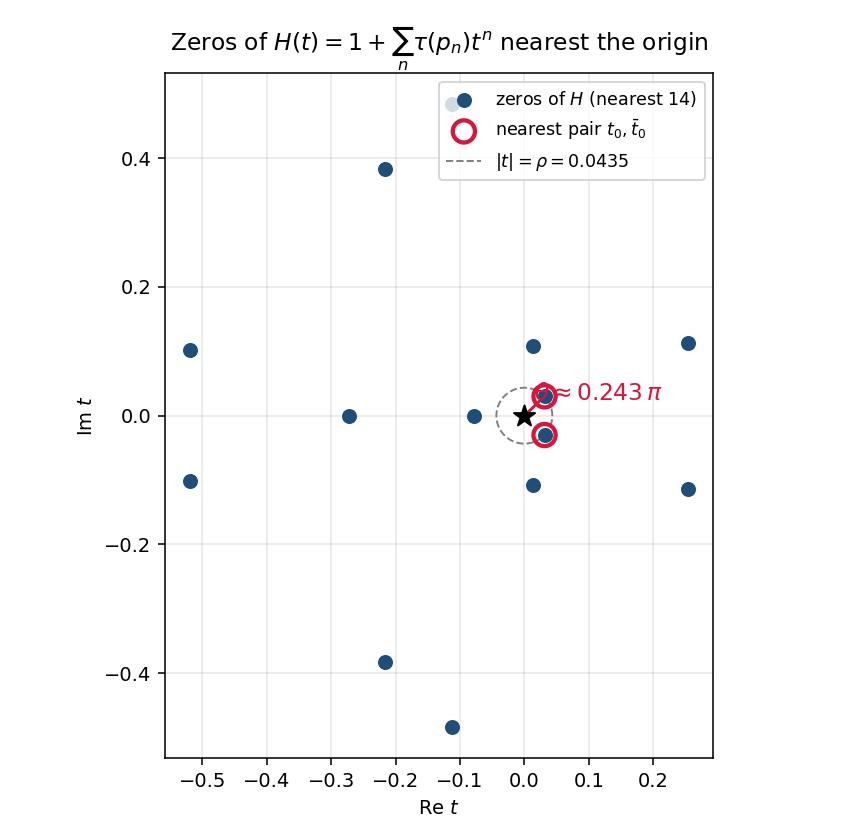
\includegraphics[width=0.66\textwidth]{fig_Hzeros.jpg}
\caption{Zeros of the truncated $H$ nearest the origin. The nearest pair $t_0,\bar t_0$
(circled) has modulus $\rho\approx0.0435$ and argument $\pm\theta\approx\pm0.2432\pi$.
These are the dominant singularities of $G=\exp\int J$.}
\label{fig:Hzeros}
\end{figure}

\section{Consequence: the coefficients grow, and carry a phase}\label{sec:growth}

A dominant singularity of $G$ at $t_0=\rho e^{i\theta}$ (with its conjugate) forces
\[
g_m \;\sim\; C\,\rho^{-m}\,\cos(m\theta+\varphi)\;\times\;(\text{slowly varying}),
\]
and the same form passes to $h_n^{(c)}$ because $e^{ct}$ is entire (it contributes no
singularity, only a convolution). Two predictions follow, both confirmed.

\emph{Growth rate.} $|g_m|^{1/m}\to 1/\rho\approx 23$. Figure~\ref{fig:growth} shows the
measured $|g_m|^{1/m}$ climbing toward this value. So the coefficients grow geometrically;
they do \emph{not} tend to finite limits. This is the decisive contrast with $h\equiv2$,
where $G(t)=1/(1-t^2)$ has its singularities \emph{on} the unit circle ($\rho=1$) at the
real points $t=\pm1$, giving bounded coefficients and the finite parity limits
$\cosh c,\sinh c$ --- the flat plateau. Here the singularity sits deep inside the disc
($\rho\approx0.04$) and off the real axis, so there is no plateau.

\emph{Phase.} The factor $\cos(m\theta+\varphi)$ makes the signed coefficients oscillate
with period $2\pi/\theta\approx 8.2$; numerically the signs of $g_m$ run in blocks
$\dots{+}{+}{+}{+}{-}{-}{-}{-}\dots$ of length about four.

\begin{figure}[H]
\centering
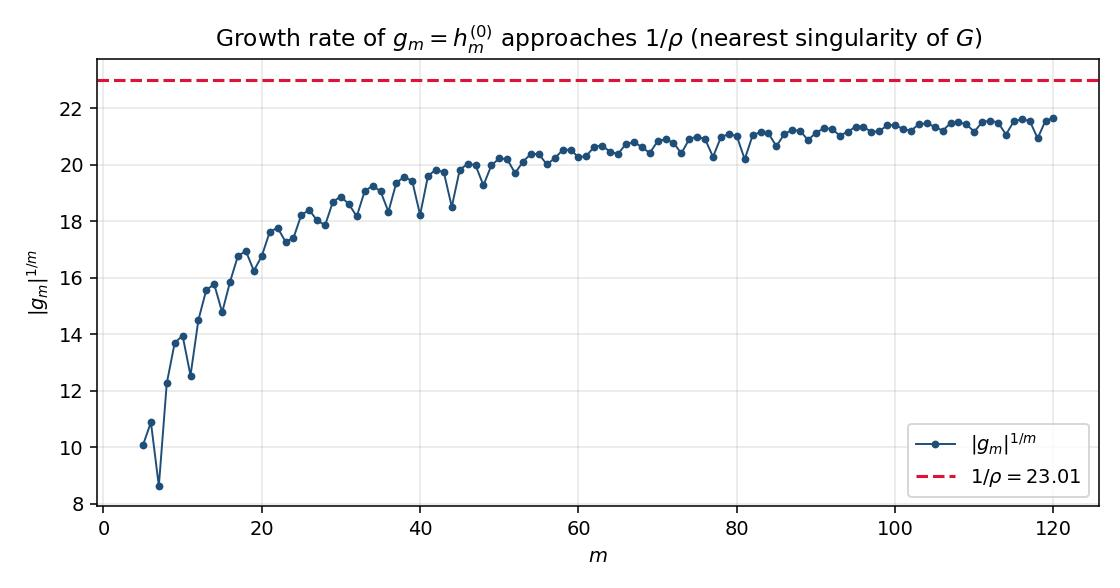
\includegraphics[width=0.82\textwidth]{fig_growth.jpg}
\caption{The growth rate $|g_m|^{1/m}$ of $g_m=h_m^{(0)}$ rises toward $1/\rho\approx23$,
the reciprocal modulus of the nearest zero of $H$. The coefficients grow geometrically;
they do not converge.}
\label{fig:growth}
\end{figure}

\section{The oscillation of \texorpdfstring{$\mu_n^{(c)}$}{mu n}}\label{sec:osc}

The link from coefficients to the plotted minimum modulus is the product of the roots. Since
$\chi_n^{(c)}$ is monic, the product of its roots equals $(-1)^n\chi_n^{(c)}(0)=n!\,h_n^{(c)}$,
so
\[
\mu_n^{(c)}\;=\;\frac{n!\,\bigl|h_n^{(c)}\bigr|}{\displaystyle\prod_{\rho_i\neq\min}|\rho_i|}.
\]
The denominator (the product of the other roots --- the bulk ring) varies smoothly with $n$,
so the \emph{oscillation} of $\mu_n^{(c)}$ comes from $\bigl|h_n^{(c)}\bigr|$. Two things
result.

First, the magnitude $\bigl|h_n^{(c)}\bigr|$ oscillates at \emph{half} the period of the
signed coefficient, $\pi/\theta\approx 4.1$, because $|\cos|$ has half the period of
$\cos$. This is the ``period~$4$'' seen directly in the plots.

Second, $\bigl|h_n^{(c)}\bigr|$ dips toward zero exactly at the sign changes of $h_n^{(c)}$
(where the cosine passes through zero), and at those $n$ the root nearest the origin must
plunge inward to keep the product small. Figure~\ref{fig:dips} shows this: the dips of
$\mu_n^{(1)}$ and the dips of $\bigl|h_n^{(1)}\bigr|^{1/n}$ both sit on the dashed
sign-change lines. The deep dip $\mu_{40}^{(1)}=0.435$ is the $+\!\to\!-$ sign change of
$h_n^{(1)}$.

\begin{figure}[H]
\centering
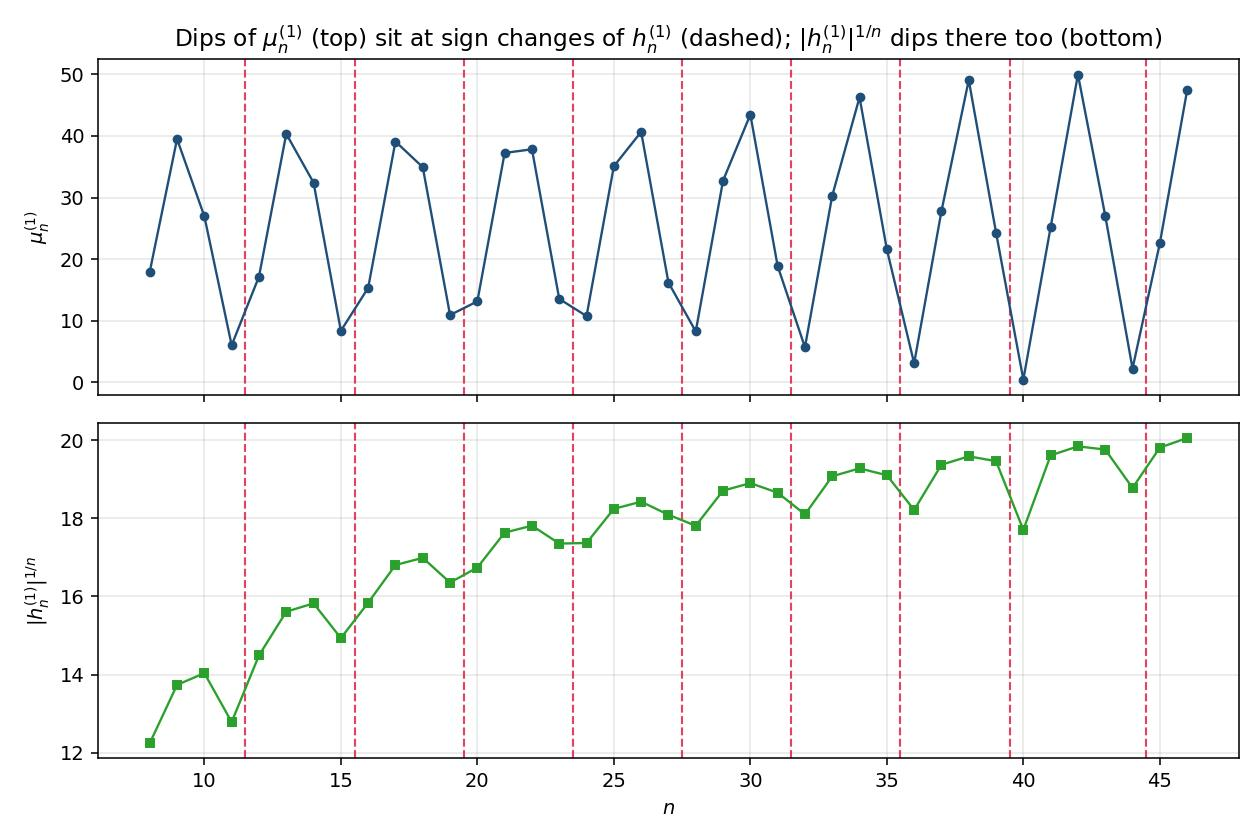
\includegraphics[width=\textwidth]{fig_dips.jpg}
\caption{Top: $\mu_n^{(1)}$. Bottom: $|h_n^{(1)}|^{1/n}$. Dashed lines mark the sign changes
of $h_n^{(1)}$. The minimum modulus dips precisely where $h_n^{(1)}$ changes sign --- the
oscillation is the magnitude of the deformed coefficient, transmitted through the product of
the roots.}
\label{fig:dips}
\end{figure}

\section{The two scales}\label{sec:scales}

The plots show a fast oscillation filling a band and a slow scalloped envelope. Both are the
single number $\theta/\pi\approx0.2432$, read at two resolutions. Its nearby rational is
$\theta/\pi\approx 9/37$, so $37\,\theta\approx 9\pi$: after about $37$ steps the phase
$n\theta$ advances by an odd multiple of $\pi$ and the magnitude pattern nearly recurs. The
fast scale $\pi/\theta\approx4.1$ fills the band; the near-recurrence at $\approx37$ is the
envelope. In dynamical language $\theta/\pi$ plays the role of a rotation number, and the
two visible scales are its first rational approximations.

\section{Contrast, and boundaries}\label{sec:boundaries}

The whole difference between the $h\equiv2$ plateau and the $\tau$ oscillation is the
location of one singularity of $G$:
\begin{center}
\begin{tabular}{lll}
\toprule
 & $h\equiv2$ & $h_n=\tau(p_n)$\\
\midrule
nearest singularity of $G$ & $t=\pm1$ (on the circle) & $t_0\approx0.0435\,e^{\pm0.243\pi i}$ (inside)\\
modulus $\rho$ & $1$ & $\approx0.0435$\\
argument & $0,\ \pi$ (real) & $\approx0.243\pi$ (complex)\\
coefficients $h_n^{(c)}$ & bounded, limits $\cosh c,\sinh c$ & grow like $\rho^{-n}$, no limit\\
$\mu_n^{(c)}$ & flat plateau (period $2$) & oscillation, period $\pi/\theta\approx4$\\
\bottomrule
\end{tabular}
\end{center}

\noindent The one-line summary: \emph{the deformed coefficients grow like $\rho^{-n}$ and
carry a phase $e^{in\theta}$ inherited from the nearest zero $t_0=\rho e^{i\theta}$ of $H$;
because $t_0$ lies inside the disc with complex argument, there is no plateau but a wave of
frequency $\theta$, and $\mu_n^{(c)}$ traces its half-period magnitude envelope, dipping to
near-zero at each sign change of $h_n^{(c)}$.}

\begin{remark}[what is and isn't established]
The asymptotic form is leading order: it keeps only the dominant conjugate pair $t_0,\bar
t_0$; the subdominant zeros at $0.078,0.108,\dots$ add corrections. The passage from
$\bigl|h_n^{(c)}\bigr|$ to $\mu_n^{(c)}$ assumes the bulk-root product is smooth in $n$ ---
strongly supported by Figure~\ref{fig:dips}, not proved. And $\rho$, $\theta$, the value
$\theta/\pi\approx9/37$, and the $\approx37$ envelope are all measured from a truncated $H$
at modest $n$. Finally, the open quantitative question --- whether $\mu_n^{(c)}$ is bounded
away from $0$ --- becomes sharp here: it asks how close $n\theta+\varphi$ comes to an odd
multiple of $\pi/2$, i.e.\ how well $\theta/\pi$ can be approximated by half-integers over
denominators up to $n$. That is a statement about the arithmetic of the single number
$\theta/\pi$.
\end{remark}

\end{document}
